\documentclass[a4paper,11pt]{article}
\usepackage[margin=2cm]{geometry}
\usepackage{anysize}
\usepackage[pdftex]{graphicx}
\usepackage{subfigure}
\usepackage[hyphens]{url}
\usepackage{listings}
\usepackage{textcomp}
\usepackage{wrapfig}
\usepackage{fixltx2e}
\usepackage{color}
\usepackage{fancyhdr}
\usepackage[nodayofweek]{datetime}
\usepackage[small,compact]{titlesec}
\usepackage[pdfborder=0]{hyperref}
\longdate

\definecolor{dkgreen}{rgb}{0,0.6,0}
\definecolor{gray}{rgb}{0.5,0.5,0.5}
\definecolor{mauve}{rgb}{0.58,0,0.82}
\definecolor{light-gray}{gray}{0.95}


\lstset{ %
  language=Java,                % the language of the code
  basicstyle=\footnotesize,           % the size of the fonts that are used for the code
  numbers=left,                   % where to put the line-numbers
  numberstyle=\tiny\color{gray},  % the style that is used for the line-numbers
  backgroundcolor=\color{light-gray},
  stepnumber=1,                   % the step between two line-numbers. If it's 1, each line 
                                  % will be numbered
  numbersep=5pt,                  % how far the line-numbers are from the code
  showspaces=false,               % show spaces adding particular underscores
  showstringspaces=false,         % underline spaces within strings
  showtabs=false,                 % show tabs within strings adding particular underscores
  tabsize=2,                      % sets default tabsize to 2 spaces
  captionpos=b,                   % sets the caption-position to bottom
  breaklines=true,                % sets automatic line breaking
  breakatwhitespace=false,        % sets if automatic breaks should only happen at whitespace
  title=\lstname,                   % show the filename of files included with \lstinputlisting;
                                  % also try caption instead of title
  keywordstyle=\color{blue},          % keyword style
  commentstyle=\color{dkgreen},       % comment style
  stringstyle=\color{mauve},         % string literal style
  escapeinside={\%*}{*)},            % if you want to add a comment within your code
}

\setlength{\parskip}{10pt} 
\setlength\parindent{0pt}
\pagestyle{fancyplain}
\fancyhf{}
\lhead{\fancyplain{}{M.Sc.\ Group Project Report}}
\rhead{\fancyplain{}{\today}}
\cfoot{\fancyplain{}{\thepage}}


\title{Twitter for traffic\\\Large{--- Final Report ---}}
\author{Porfyrios Vasileiou, Marianna Polatoglou, Afxentios Hadjiminas,\\
        Panagiotis Tsirigotis, Hanguang Zhou, John Flanagan.\\
       \{pv311, mp1911, ah2411, pt1111, hz511, jf311.\}@doc.ic.ac.uk\\ \\
       \small{Supervisors: Dr.\ Emil Lupu, Dr.\ Alessandra Russo, Dr.\ Luke Dickens}\\
       \small{Course: CO533, Imperial College London}
}

%Report details http://www.doc.ic.ac.uk/~cristic/teaching/MScGroupProj/

\begin{document}
\maketitle
\pagebreak
\tableofcontents
\pagebreak
\section{Introduction}
	Twitter for traffic aims to provide the mobile user with an application for assessing traffic disruptions as they evolve. To provide this insight, the application will present the user with curated traffic disruptions augmented with social knowledge of the event harvested from a social network. In addition to this curated list of traffic disruptions, Twitter for traffic will also extract clusters of disruption reports from social networks to identify new disruptions.

To successfully achieve the project goals, the development will encompass an understanding from many areas of computer science. Aspects of this project include data mining, social network analysis, mobile application development, document classification and geographical information systems. Analysing the social and curated datafeeds to identify new disruption events will be a particularly interesting undertaking. From the onset there are many unknowns relating to the data analysis, relating to the quantity of traffic related messages and quality of the content. 


\pagebreak
\section{Specifications}
	\subsection{Server}

\subsection{Client}


\pagebreak
\section{Design}
	
\subsection{System overview}
	\begin{center}
	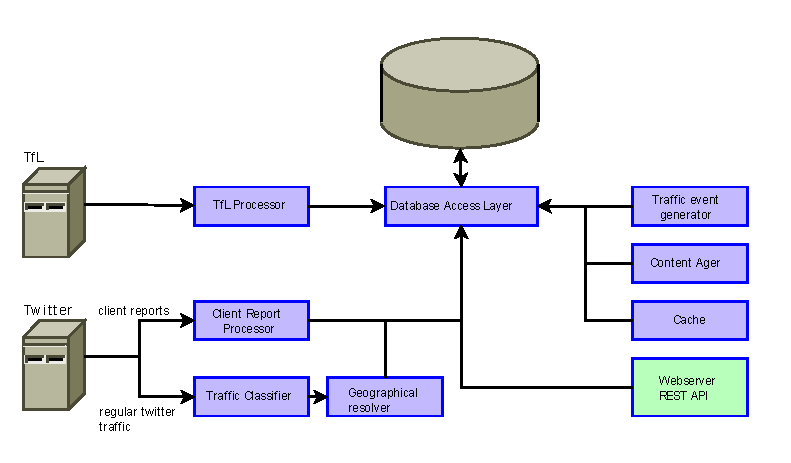
\includegraphics{images/high_level_system_arch.pdf}
	\end{center}
\subsection{Server}
  
\subsubsection{Data acquisition}
\subsubsection{Data analysis}
\subsubsection{Storage}
\subsubsection{Interface}


\subsection{Client}
  \begin{figure}[htb]
\centering
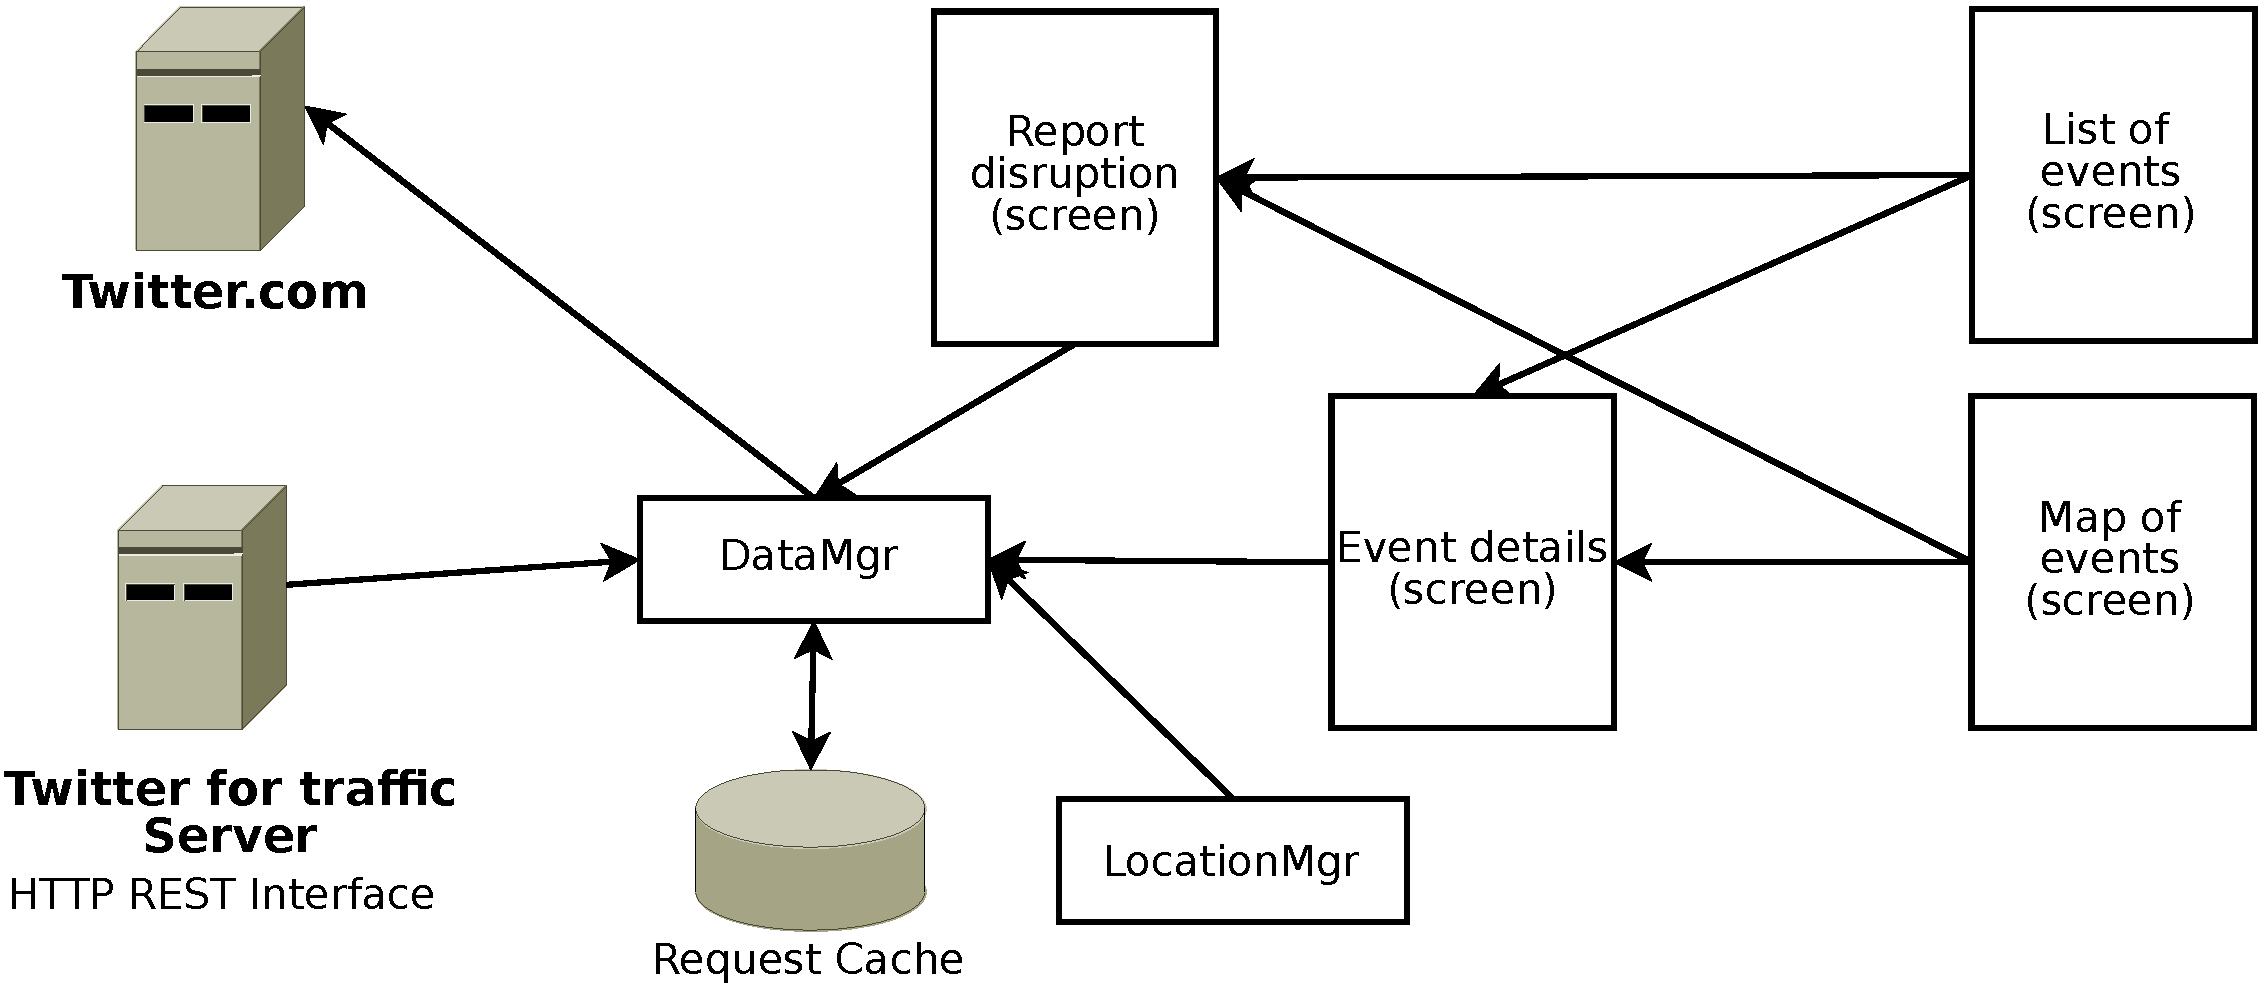
\includegraphics[width=0.9\textwidth]{images/design/client/client_high_level_layout.pdf}
\caption{High level client design}
\label{fig:client_design}
\end{figure}



\subsubsection{User interface}
\subsubsection{Request caching}




\pagebreak
\section{Document Classification}
	Document classification is a way to categorize documents or pieces of text. By examining the words in a piece of text, classifiers can decide, after the training what class label to assign to it. A binary classifier decides between two labels, such as traffic or non-traffic. The text can either be one label or the other, but not both, whereas a multi-label classifier can assign one or more labels to a piece of text. For the particular project, because it was only required to label the tweets as traffic or as non-traffic, the binary classifier has been chosen.

Two approaches for the automatic document classification exist: supervised document classification and unsupervised classification (clustering) \cite{Liu}.  The supervised classification requires training data in order to be able to classify the data. This classification works by learning from labelled feature sets, or training data, to later classify an unlabelled text, or a feature set. A feature set is basically a key-value mapping of feature names to feature values. In the case of text classification, the feature names are usually words or blocks of words, and the values are all True. As the texts may have unknown words, and the number of possible words may be very large, words that do not occur in the text are omitted, instead of being included in a feature set with the value False.

On the other hand, unsupervised classification instead of training data uses several algorithms, mainly clustering algorithms, to classify text. The unsupervised classification starts from a certain point and its algorithms try in iterative ways to reach a stable configuration that makes sense. Therefore, it may require a large amount of time to reach this configuration and the time was of the essence because of the strict project time restrictions. Additionally, the results of the unsupervised classification vary widely and may be completely off if the first steps are wrong.

The team decided to adopt the supervised classification because it is a more stable technique and it can be used as soon as the classifier is trained. It is only needed to gather the training data, train the classifier and then the classifier is ready to start classifying. After the decision of the classifier, it was necessary to apply several text normalizations on the data. 

\subsection{Text Normalization}
Text normalization is the way to eliminate the low information features, the words that don't offer useful information to the classifier. The elimination of those low information features provides to the model clarity by removing noisy data. Additionally it reduces the possibility of over-fitting by training the classifier with unnecessary data. By using the higher information features, the performance is being increased while the size of the model is being decreased, which results in less memory usage along with faster training and classification. This normalization was being applied on the labelled tweets before the classifier training and is continue being applied on the newly fetched tweets as well. Using this pre-processing on the tweets the accuracy of the classifier has been increased. 

The below text normalazation techniques are being applied on the tweets before the classification.
\begin{itemize}
\item Convert URL links to a more redable way.\\ 
This has been done by using a regular expression to recognize the link. After that the domain is being extracted from the URL and it replaces the link itself. 
\item Convert emoticons into words.\\ 
The next step is to replace the emoticons with a global name so they will not be deleted during the punctuation removal. That is important because the emoticons offer useful information during the classification. For this reason, the team has integrated a script which is responsible on finding those emoticons, assign them to a group of emoticons and replace them with the name of the group. Four groups of emoticons have been created:Very Happy, Happy, Sad, Very Sad. 
\item Remove the punctuations.\\
The team has accomplished that by creating a regular expression which represents all the possible punctuations. 
\item Convert all letters to lower case.
\item Tokenise the tweet into words.
\item Group together the different inflected forms of a word into a single item.\\
This has been done by applying lemmanization on the tokenised text. Lemmanization removes and replaces word suffixes to arrive at a common root form of the word in order to group up the common words. This method has been chosen over the stemming, because lemma is a canonical set of words, instead of the stem which in many cases is not a real world. 
\item Find the bigrams collocations.\\
Bigrams are less common than most individual words, so including them in training data increases the classifier accuracy. 
\end{itemize}

\subsection{Classifiers}
The next step was to investigate several supervised classification algorithms. The methods Support Vector Machines and Naive Bayes have been chosen for this purpose. Those two algorithms have been selected because of a number of factors. Firstly, Naive Bayes train very quickly since it requires only a single pass on the data to compute the normal probability density function. It also requires little storage space during the training and classification stages: the strict minimum is the memory needed to store the prior and conditional probabilities. Additionally Naive Bayes is very transparent, as it is easily grasped by users and it provides a discrete probability for each tweet helping the ranking of the tweets. Naive Bayes is considered to have high bias, because it assumes that the dataset under consideration can be summarized by a single probability distribution and that Naive Bayes model is sufficient to discriminate between classes. This high bias usually generates simple, highly constrained models. On the other hand, SVM is considered to be one of the most accurate classifier. However for the SVM, a large sample size is required in order to achieve its maximum prediction accuracy whereas Naive Bayes may need a relatively small dataset.

\subsubsection{Naive Bayes}
Given a set of objects, each of which belongs to a known class, and each of which has a known vector of variables, the aim is to construct a rule which will allow the assigning of future objects to a class, given only the vectors of variables describing the future objects. Problems of this kind, called problems of supervised classification, are ubiquitous, and many methods for constructing such rules have been developed. One method is the Naive Bayes Reasoning. This is a well-established Bayesian method primarily formulated for performing classification tasks. Given its simplicity Naive Bayes models are effective classification tools that are easy to use and interpret. Naive Bayes is particularly appropriate when the dimensionality of the independent space. For the reasons given above, Naive Bayes can often outperform other more sophisticated classification methods. A variety of methods exist for modelling the conditional distributions of the inputs including normal, lognormal, gamma, and Poisson \cite{Barber}. 

This classifier has been created using the "Bag of Words" model and the NLTK suites of libraries. NLTK is the Natural Language Toolkit, a comprehensive Python library for natural language processing and text analytics. It was decided to use the Natural Language Toolkit because of its simplicity, consistency, extensibility and its modularity. Additionally some of the members had already experience with it and they were aware of its accuracy. Furthermore, it was decided the usage of the "Bag of Words" feature extraction because it's a very accurate method, especially for binary classification. Text feature extraction is the process of transforming what is essentially a list of words into a feature set that is usable by a classifier. The NLTK Naive Bayes classifier expects dictionary style feature sets, so the text should be transformed into a dictionary. The "Bag of Words" model is a well-known method for representing documents, which ignores the word orders \cite{Bird}\cite{Perkins}. It constructs a word dictionary from all the words of an instance where every word gets the value True. An instance is a single feature set. It represents a single occurrence of a combination of features. A labelled feature set is in fact an instance with a known class label that we can use for training or evaluation.

As it has discussed previously, for the training of the classifier it's required a labelled data. To accomplish that, a simple script for manually labelling was created. This script was being executed on a temporary table on the database which was containing raw, unlabelled, tweets. During the execution it was presenting random tweets from this table and the user was able to press four buttons in order to label the tweets as traffic (personalized tweets about traffic), non-traffic, unclear and bot (tweets about traffic from official sites). After the gathering of one and a half thousand of traffic-about tweets, the table in which the labelled tweets were being stored was used to train the classifier.

\subsubsection{Support Vector Machines}
The second supervised learning method that it was fully integrated and tested is the Support Vector Machines (SVM). This is a method that performs regression and classification tasks by constructing nonlinear decision boundaries. Because of the nature of the feature space in which these boundaries are found, Support Vector Machines can exhibit a large degree of flexibility in handling classification and regression tasks of varied complexities. There are several types of Support Vector models including linear, polynomial, RBF, and sigmoid.

In this project PyML\cite{website:pyml} was used to implement SVM
classification. The results of this algorithm did not show much improvement
compared to Naive Bayes classification. Also the library seems to be at an
early stage which makes it more difficult to use. Since the accuracy does not
change, the use of Naive Bayes was decided by the group.

\subsection{Classifier Evaluation} 
Machine learning algorithms induce classifiers that depend on the training set. So there is a need for evaluation and statistical testing to assess the expected error rate of a classification algorithm. Additionally evaluation is crucial to compare the expected error rates of two classification algorithms to be able to say which one is better. Evaluation can also be used as a guide for future improvements on the model. In order to evaluate the classifier several techniques have been used. The first technique is to generate a test set of tweets which their labels are already known. This test set has to be distinct from the train set which has been used to train the classifier. It is then being labelled by the classifier and the labels that it decides are being compared with their correct labels. The second technique is to calculate the accuracy of the classifier which measures the percentage of inputs in the test set that the classifier correctly labelled. To accomplish this, the build-in function of the package NLTK \emph{nltk.classify.accuracy()} has been used.

Additionally techniques have been implemented in order to get moreaccurate evaluations and avoid possible `overfitting'. There is a chance the classifier will become more accurate in the train set and less accurate in the test set with some parameter changes. This is when an "over-fitting" is occurs to the train set. 

The first of these methods is the K-Fold Cross Validation. The dataset is split each time into K equally sized subsets, training and testing datasets, and then in n-th iteration (n=1..k) the n-th subset(testing set) is used for testing the classifier that has been built on all other remaining subsets. To present the result of this method the Confusion Matrix, which is a visualization tool typically used to present the results attained by a learner, has been created. Each column of the matrix represents the instances in a predicted class, while each row represents the instances in an actual class. Thus, the diagonal entries indicate labels that were correctly predicted, and the off-diagonal entries indicate errors. One benefit of a confusion matrix is that it is easy to see if the system is confusing two classes.

The Precision and Recall Rates can be calculated in order to ensure the results from the previous method. Recall describes the completeness of the classification. It is defined as the portion of the traffic tweets versus retrieved by the classifier the number of existing traffic tweets. Precision defines the actual accuracy of the classification. It is defined as the portion of the traffic tweets exist in the total number of tweets classified. The recall and the precision can be derived from the confusion matrix by applying the following formulas:

\[ Precision\textsubscript{A} = tp\textsubscript{A}/(tp\textsubscript{A}+e\textsubscript{BA}+e\textsubscript{CA}) \]

\[ Recall\textsubscript{A} = tp\textsubscript{A}/(tp\textsubscript{A}+e\textsubscript{AB}+e\textsubscript{AC}) \]

Where the values "tp" and "e" are the elements of the confusion matrix as it can been seen on the figure~\ref{fig:confisionMatixCalc}.

\begin{figure}[h!]
\begin{center}
\begin{tabular}{| l || c | c | c | }
    \hline
        & A & B & C  \\ \hline \hline
        A & tp\textsubscript{A} & e\textsubscript{AB} & e\textsubscript{AC} \\ \hline
        B & e\textsubscript{BA }& tp\textsubscript{B} & e\textsubscript{BC} \\\hline
        C & e\textsubscript{CA} & e\textsubscript{CB} & tp\textsubscript{C} \\\hline
    \end{tabular}
	\caption{A simple confusion matrix}
    \label{fig:confisionMatixCalc}
\end{center}
\end{figure}

While recall and precision rates can be individually used to determine the quality of a classifier, it is often more convenient to have a single measure to do the same assessment. The F\textsubscript{1} measure combines the recall and precision rates in a single equation:

\[ F\textsubscript{1} = 2*\frac{precision*recall}{precision+recall} \]

The labelled data was consisting of an unbalance data, 1500 traffic tweets and 14505 non-traffic tweets, two different trainings have been executed and tested. 

Firstly, the classifier was trained with 1000 traffic and 1000 non-traffic tweets. Then it was tested with 500 traffic and 500 non-traffic tweets. The metrics for this training are the following. 

Accuracy of the classifier:   0.870000

Traffic precision:\hspace{15.5 mm}              0.842592592593\\
Traffic recall:\hspace{21.2 mm}                             0.91\\
Traffic F-measure:\hspace{12.8 mm}             0.875\\

Non-Traffic precision:\hspace{7.2 mm}        0.902173913043\\
Non-Traffic recall:\hspace{13 mm}            0.83\\
Non-Traffic F-measure:\hspace{4.6 mm}       0.864583333333\\

\begin{figure}[h!]
\begin{center}
    \begin{tabular}{| l || c | c | }
    \hline
          & Non-Traffic & Traffic \\ \hline \hline
         Non-Traffic & 83.0\% & 17.0\% \\ \hline
         Traffic & 9.0\% & 91.0\% \\ \hline
    \end{tabular}
    \caption{Confusion Matrix with 1000 traffic and 1000 non-traffic tweets.}
    \label{fig:confusionMatrix1}
\end{center}
\end{figure}	

Secondly, the classifier was trained with 1000 traffic and 9670 non-traffic tweets. Afterward it was tested with 500 traffic and 4835 non-traffic tweets. The metrics for this training are the following. 

Accuracy of the classifier:   0.862605

Traffic precision:\hspace{15.5 mm}            0.401019541206\\
Traffic recall:\hspace{21.2 mm}               0.944\\
Traffic F-measure:\hspace{12.8 mm}         0.562909958259\\

Non-Traffic precision:\hspace{7.2 mm}         0.993265993266\\
Non-Traffic recall:\hspace{13 mm}           0.854188210962\\
Non-Traffic F-measure:\hspace{4.6 mm}         0.918492160569\\

\begin{figure}[h!]
\begin{center}
    \begin{tabular}{| l || c | c | }
    \hline
          & Non-Traffic & Traffic \\ \hline \hline
        Non-Traffic & 85.4\% & 14.6\% \\ \hline
        Traffic & 5.4\% & 94.6\% \\ \hline
    \end{tabular}
    \caption{Confusion Matrix with 1000 traffic and 9670 non-traffic tweets.}
    \label{fig:confusionMatrix1}
\end{center}
\end{figure}
	
It can been observed from the confusion matrices, with the first training the classifier has been achieved a rather bad accuracy since 19\% of the non-traffic tweets are being classified wrong and 9\% of the traffic tweets are being classified wrong. On the other hand, with the second training the traffic tweets error has been almost halved to 5\% resulting a more accurate classification for the traffic tweets even if the global accuracy dropped by 1\%. That means the classifier may classified some traffic tweets as non-traffic but it classified much less non-traffic tweets as traffic.So ita has been decide from the team to train the Naive Bayes classifier with all the labelled data. Note that all the above results have been taken after the implementation of the normalization. During the first evaluation, before the pre-processing, the accuracy of the classifier was 77\%. However after the application of the normalization techniques the accuracy has been increased by 10\%!

A strong motivation for the creation of this project was the previous work of Dr.Luke Dicken in the same field. Having that in mind, is important to compare the accuracy of our classifier and the efficient of our server with his work. So in addition to the previous evaluation results, several metrics have been calculated in order to find the efficient of the classifier and the server. Those metrics are being presented in the figures below.

\begin{figure}[h!]
\begin{center}
    \begin{tabular}{| c | c | c | }
    \hline
        Total Number of Tweets  & Non-Traffic & Traffic \\ \hline 
        71036 & 68096(95.86\%) & 2940(4.14\%) \\ \hline
    \end{tabular}
    \caption{Comparison of Traffic and Non-Traffic Tweets.}
    \label{fig:metrics1}
\end{center}
\end{figure}
	
\begin{figure}[h!]
\begin{center}
    \begin{tabular}{| c | c | c | }
    \hline
        Geo-Tagged  & Geo-Tagged Genuine & Geo-Tagged from the 
Geolocation Resolver \\ \hline 
        314(10.68\%) & 136(4.63\%) & 178(6.05\%) \\ \hline
    \end{tabular}
    \caption{Tweets with geolocation from the 2940 traffic tweets.}
    \label{fig:metrics2}
\end{center}
\end{figure}


\begin{figure}[h!]
Overall inferred rates:
\begin{center}
    \begin{tabular}{| l || c | c | c |}
    \hline
        & Filtered & Traffic & Geo-Tagged and Traffic\\ \hline \hline
        each minute & 13.3 & 0.5 & 0.06 \\ \hline
		each 5 mins & 66.7 &  2.7 & 0.3 \\ \hline
		each hour & 800 & 32.7 & 3.5 \\ \hline
    \end{tabular}
    \caption{Averages are over total 5400 minutes (90 hours) of up-time.}
    \label{fig:metrics3}
\end{center}
\end{figure}

The corresponding metrics from Dr. Luke Dicken are being presented below.

Accuracy of the classifier:   0.818750

\begin{figure}[h!]
\begin{center}
    \begin{tabular}{| l || c | c | }
    \hline
          & Non-Traffic & Traffic \\ \hline \hline
        Non-Traffic & 85.8\% & 14.2\% \\ \hline
        Traffic & 22.3\% & 77.7\% \\ \hline
    \end{tabular}
    \caption{Confusion Matrix of Dr. Luke Dicken SVM classifier.}
    \label{fig:confusionMatrixLuke}
\end{center}
\end{figure}

\begin{figure}[h!]
Overall inferred rates:
\begin{center}
    \begin{tabular}{| l || c | c | c |}
    \hline
        & Filtered & Traffic & Geo-Tagged and Traffic\\ \hline \hline
        each minute & 6.3 & 3.6 & 0.11 \\ \hline
		each 5 mins & 32 &  18 & 0.5 \\ \hline
		each hour & 380 & 220 & 6.5 \\ \hline
    \end{tabular}
    \caption{Averages are over total 160000 minutes (111 days) of up-time.}
    \label{fig:metricsLuke}
\end{center}
It can be clearly seen that comparing to Dr. Luke's classifier; the Naive Bayes classifier sacrificed the quantity to achieve the quality. Our classifier labelled less tweets as traffic, but those tweets are rather accurate. That�s important because the application�s user prefer to have less tweets for each disruption, but these tweets have to be about traffic. 
\end{figure}

	
\pagebreak
\section{Methodology}
	\subsection{Development approach} 
To begin identifying an appropriate development methodology, it was necessary to firstly understand 
the project requirements. The project requirements and features were agreed over a number of 
meetings with the primary stakeholders.

The two most preferred development methodologies were 
Scrum and XP(Extreme Programming) which are both Agile methodologies. Scrum is an agile project management technique that focuses more 
on the management of software development projects. The product is completed in a series of one to 
four week iterations, or sprints as they are called. Before each sprint, a planning meeting is held 
to determine which features will be implemented during that sprint. Similarly, XP is an agile 
methodology which is designed for small, co-located teams aiming to get quality and productivity as 
high as possible. It does this through the use of rich, short, informal communication paths with 
emphasis on skill, discipline and understanding at the personal level, minimizing all intermediate 
work products. 

It was decided amongst the group that combining characteristics form both methods 
would be the most beneficial way, merely because they are complementary. Scrum focuses on the project management 
whereas XP on the programming part.\cite{ScrumXP}

Managing efficiently the development lifecycle of the project was a very 
important task for the team to work properly. Meetings with the supervisor took place each week 
where the project progress was thoroughly discussed as well as more feasible features to be 
implemented. In addition, various issues were constantly being brought up in order to provide solutions. Except from 
the meetings with the supervisor, the team had its own weekly meeting for keeping up with what 
everyone has been doing for the last week. New tasks were also assigned to members of the team. For 
every meeting an agenda was stored in an online document containing information about the team 
members absent, location, action items and topics to be discussed. In the end of the meeting tasks 
were assigned, managed or archived using an online visual board, similar to the Scrum Board, to 
encourage a more agile development.

As regards to the XP approach, it was proved that adopting 
some of its techniques would significantly improve the development process. More specifically, pair 
programming was effectively put in use. Team members where working in pairs whenever possible to 
develop a single feature. Additionally, XP promotes test-driven development. As mentioned in the 
first report, testing would be rather difficult due to the nature of the project being partly 
research based. However, essential tests were implemented in the server to validate the classifier 
as well as blackbox tests for the correctness and responsiveness of the rest API server. 

Throughout the development, various technologies had to be used and implemented. According to each 
members skills these elements were divided in such ways to effectively use the members previous 
experience. The team was also distributed to different design aspects of the project; however, more on the 
team structure will be discussed further on.

Lastly, for achieving parallel development between the mobile client application and the server, 
a mock server API was created, as mentioned in earlier reports that was accepting http requests and 
was returning static data sets to the client. 

\subsection{Testing} 
\subsubsection{Classifier Evaluation} 
Machine learning algorithms induce classifiers that depend on the training set, and there is a need for evaluation and statistical testing to assess the expected error rate of a classification algorithm, and even compare the expected error rates of two classification algorithms to be able to say which one is better. Evaluation can also be used as a guide for future improvements on the model. In order to evaluate the classifier several techniques have been used. The first technique is to generate a test set of tweets which their labels are already known. This test set has to be distinct from the train set which has been used to train the classifier. Afterward this test set is being classified by the classifier and the labels that it decides are being compared with their correct labels. The second technique is to calculate the accuracy of the classifier which measures the percentage of inputs in the test set that the classifier correctly labelled. To accomplish this, the build-in function of the package NLTK \emph{nltk.classify.accuracy()} has been used.

Additionally some more techniques have been implemented in order to get more
accurate evaluations and avoid possible `overfitting'. Note that there is a chance the classifier will become more accurate in the train set and less accurate in the test set with some parameter changes. This is when we have reached an "overfitting" to the train set. The first of these methods is the K-Fold Cross Validation. The dataset is split each time into K equally sized subsets, training and testing datasets, and then in n-th iteration (n=1..k) the n-th subset(testing set) is used for testing the classifier that has been built on all other remaining subsets. To present the result of this method the Confusion Matrix, which is a visualization tool typically used to present the results attained by a learner, has been created. Each column of the matrix represents the instances in a predicted class, while each row represents the instances in an actual class. Thus, the diagonal entries indicate labels that were correctly predicted, and the off-diagonal entries indicate errors. One benefit of a confusion matrix is that it is easy to see if the system is confusing two classes.

Finally, the Precision and Recall Rates can be calculated in order to ensure the results from the previous method. The recall and the precision can be derived from the confusion matrix by applying the following formulas:

\[ Precision\textsubscript{A} = tp\textsubscript{A}/(tp\textsubscript{A}+e\textsubscript{BA}+e\textsubscript{CA}) \]

\[ Recall\textsubscript{A} = tp\textsubscript{A}/(tp\textsubscript{A}+e\textsubscript{AB}+e\textsubscript{AC}) \]

Where the values "tp" and "e" are the elements of the confusion matrix as it can been seen on the figure~\ref{fig:confisionMatixCalc}.

\begin{figure}[h]
\begin{center}
\begin{tabular}{| l || c | c | c | }
    \hline
        & A & B & C  \\ \hline \hline
        A & tp\textsubscript{A} & e\textsubscript{AB} & e\textsubscript{AC} \\ \hline
        B & e\textsubscript{BA }& tp\textsubscript{B} & e\textsubscript{BC} \\\hline
        C & e\textsubscript{CA} & e\textsubscript{CB} & tp\textsubscript{C} \\\hline
    \end{tabular}
	\caption{A simple confusion matrix}
    \label{fig:confisionMatixCalc}
\end{center}
\end{figure}

While recall and precision rates can be individually used to determine the quality of a classifier, it is often more convenient to have a single measure to do the same assessment. The F\textsubscript{1} measure combines the recall and precision rates in a single equation:

\[ F\textsubscript{1} = 2*\frac{precision*recall}{precision+recall} \]

Because the labelled data was consisting of 1500 traffic tweets and 14505 non-traffic tweets, two different trainings and evaluations have been integrated. 

Firstly, the classifier was trained with 1000 traffic and 1000 non-traffic tweets. Then it was tested with 500 traffic and 500 non-traffic tweets. The metrics for this training are the following. 

Accuracy of the classifier:   0.87\\

Traffic precision:\hspace{15.5 mm}              0.842592592593\\
Traffic recall:\hspace{21.2 mm}                             0.91\\
Traffic F-measure:\hspace{12.8 mm}             0.875\\

Non-Traffic precision:\hspace{7.2 mm}        0.902173913043\\
Non-Traffic recall:\hspace{13 mm}            0.83\\
Non-Traffic F-measure:\hspace{4.6 mm}       0.864583333333\\

\begin{figure}[h]
\begin{center}
    \begin{tabular}{| l || c | c | }
    \hline
          & Non-Traffic & Traffic \\ \hline \hline
         Non-Traffic & 41.5\% & 8.5\% \\ \hline
         Traffic & 4.5\% & 45.5\% \\ \hline
    \end{tabular}
    \caption{Confusion Matrix with 1000 traffic and 1000 non-traffic tweets.}
    \label{fig:confusionMatrix1}
\end{center}
\end{figure}	

Secondly, the classifier was trained with 1000 traffic and 9670 non-traffic tweets. Afterward it was tested with 500 traffic and 4835 non-traffic tweets. The metrics for this training are the following. 

Accuracy of the classifier:   0.862605435801

Traffic precision:\hspace{15.5 mm}            0.401019541206\\
Traffic recall:\hspace{21.2 mm}               0.944\\
Traffic F-measure:\hspace{12.8 mm}         0.562909958259\\

Non-Traffic precision:\hspace{7.2 mm}         0.993265993266\\
Non-Traffic recall:\hspace{13 mm}           0.854188210962\\
Non-Traffic F-measure:\hspace{4.6 mm}         0.918492160569\\

\begin{figure}[h]
\begin{center}
    \begin{tabular}{| l || c | c | }
    \hline
          & Non-Traffic & Traffic \\ \hline \hline
        Non-Traffic & 77.4\% & 13.2\% \\ \hline
        Traffic & 0.5\% & 8.8\% \\ \hline
    \end{tabular}
    \caption{Confusion Matrix with 1000 traffic and 9670 non-traffic tweets.}
    \label{fig:confusionMatrix1}
\end{center}
\end{figure}
	
It can been observed from the confusion matrices, with the first training the classifier has been achieved a rather bad accuracy since 19\% of the non-traffic tweets are being classified wrong and 9\% of the traffic tweets are being classified wrong. On the other hand, with the second training the traffic tweets error has been almost halved to 5\% resulting a more accurate classification for the traffic tweets even if the global accuracy dropped by 1\%. That means the classifier may classified some traffic tweets as non-traffic but it classified much less non-traffic tweets as traffic. Note that all the above results have been taken after the implementation of the normalization. During the first evaluation, before the pre-processing, the accuracy of the classifier was 77\%. However after the application of the normalization�s techniques the accuracy has been increased by 10\%!

As it has been mentioned before, a strong motivation for the creation of this project was the previous work of Dr. Luke Dicken in the same field. Having that in mind, it has been considered necessary to compare the accuracy of the classifier and the efficient of the server with his work. So in addition to the previous evaluation results, several metrics have been calculated in order to find the efficient of the classifier and the server. Those metrics are being presented in the figures below.

\begin{figure}[h]
\begin{center}
    \begin{tabular}{| c | c | c | }
    \hline
        Total Number of Tweets  & Non-Traffic & Traffic \\ \hline 
        71036 & 68096(95.86\%) & 2940(4.14\%) \\ \hline
    \end{tabular}
    \caption{Comparison of Traffic and Non-Traffic Tweets.}
    \label{fig:metrics1}
\end{center}
\end{figure}
	
\begin{figure}[h]
\begin{center}
    \begin{tabular}{| c | c | c | }
    \hline
        Geo-Tagged  & Geo-Tagged Genuine & Geo-Tagged from the 
Geolocation Resolver \\ \hline 
        314(10.68\%) & 136(4.63\%) & 178(6.05\%) \\ \hline
    \end{tabular}
    \caption{Tweets with geolocation from the 2940 traffic tweets.}
    \label{fig:metrics2}
\end{center}
\end{figure}


\begin{figure}[h]
Overall inferred rates:
\begin{center}
    \begin{tabular}{| l || c | c | c |}
    \hline
        & Filtered & Traffic & Geo-Tagged and Traffic\\ \hline \hline
        each minute & 13.3 & 0.5 & 0.06 \\ \hline
		each 5 mins & 66.7 &  2.7 & 0.3 \\ \hline
		each hour & 800 & 32.7 & 3.5 \\ \hline
    \end{tabular}
    \caption{Averages are over total 5400 minutes (90 hours) of up-time.}
    \label{fig:metrics3}
\end{center}
\end{figure}


\subsubsection{Functional/Integration Testing}
One of the most important parts of the project was the server API interface. A lot of requests will 
be coming from the mobile application and it must be confirmed that the server interface can handle 
them but also return the expected results using the expected format. In order to test the server 
interface the Apache JMeter desktop application was used. This software is designed to load test 
functional behaviour and measure the performance of static and dynamic recourses. Using JMeter 
proved to be a very effective way to test the servers interface. Various test plans where created 
testing every GET or POST request available to use through the API. These plans where created for 
both the server and the mock server that are running on ports 55004 and 55003 accordingly. More 
tests were implemented to ensure that the server was returning the correct messages and response 
codes when it was encountering an error. In addition, invalid requests to the server had also been 
checked for error handling and if the error messages were displayed correctly into the screen. For 
each request, the content-type was also checked if it evaluates as JSON. This process was really 
helpful because it was very easy later on to check whether new features implemented or code 
refactoring were actually breaking the API. All the test plan configuration settings have been saved 
in the project repository as a .jmx file. 

\subsubsection{Unit Testing} 



\pagebreak
\section{Group Work}
	\subsection{Team Structure} 
Before starting working on the project, the team structure had to be defined. Most importantly, we had to 
agree who would be the leader of the group whose main responsibility was coordinating the tasks amongst the 
team members. At the early stages of the project, all features were researched in order to 
determine their feasibility and to estimate the amount of work required for each one. Next, according to 
each members previous experience and expertise, the team was divided into 3 subgroups, each one assigned to 
a different aspect of the project. Only one person was responsible for designing the client application, while
we provisioned the team manpower to the server. Two members were allocated to creating and training 
the classifier and two more focused on the implementation of the server. The last person was rotating through 
all the aspects of the project, providing help when needed. Every team member was expected to contribute 
at least 10 hours per week on this group project.\\ 

\subsection{Collaboration Tools} 
Project management is a vital part of any project. There exist a series of tools that enable effective team 
collaboration during a project. One of these tools is \emph{Trello} which gives access to a visual board 
that displays the ongoing tasks. This concept is very similar to the Scrum board. All these tasks 
are represented as cards with labels, priorities and deadlines assigned to 
team members. In this visual board we have the lists for separating the tasks such as `To Do', `Started', `Review' and `Done this week'. 
Additionally, six labels were created with different colours to identify their kinds of tasks like data, 
documentation, server, android app, text analysis and meeting preparation. Future tasks were 
discussed at the weekly group meeting and assigned to the `To Do' list. A team member who started a task that he was responsible of, 
would drag this card to the `Started' list to inform the rest group members that this task was currently being processed. 
After a task was finished, the card was moved to the `Review' list so other members would evaluate it. 
On every group meeting, reviewed tasks were transferred to the `Done this week' list and in the end of the meeting they were
archived.\\ 
Another tool that has been used for this project was Github. Github is used as our revision control system to manage 
the source-code and documentation. It enables multiple team members to work on a set of files, 
ensuring that changes will not get lost. Other features include version tracking, verifiable histories, integration with deployment, 
test and code review systems and the ability to add rules to enforce corporate policy and process. \\
When a team member makes changes to a file in the project, his next step is to commit it and push it to the repository. 
This updates the state of the project and the other team members can pull and receive the updated project repository. 
Github stores the history of all the changes so that individuals can compare or revert 
to previous versions of the project. Furthermore, Github provides a `Wiki' feature that enables team members 
to add description or instructions for specific components that are implemented in the project.\\
From the beginning of the project it was agreed that all data will exist outside of the repository. This was enforced by 
policy and by using a `.gitignore' file of the repository to list file types to be not tracked.


% A repository called 'Twitter for Traffic' is created in 
% Github. The project is divided into several parts. We create a 'classifier' file for data mining and 
% 'data\_acquisition' file to retrieve tweets and TfL data. 'mobile\_client' folder is built for 
% Android application development. 'mock\_server' and 'server' folders are platform which is providing 
% and processing data for mobile client. A folder called 'scrapbook' is created for each members to 
%store source codes and test each unit function.

	
\pagebreak
\section{Final Product}
	\subsection{Achieved goals and difficulties}
The specifications and which of them were implemented or not is described in
Section 2. All the features from the minimum specifications were imlemented
fully. Also, there were features that were not in the specifications and were
implemented nonetheless.

A profanity checker was included, as stated in Section 4.2.1, to check if the social data included any
cursing words. Every time a tweet is processed before entering the database
there is a profanity check and it is marked accordingly. By default the
application does not use the profanity checker, but the user can enable it from
the settings.

Soundex algorithm was implemented as well, as stated in Section 4.2.2, in order to enhance the possibility to identify
a location just from the text of a tweet. This algorithm understands
misspelled words, and so gives the ability to search for street names that may
be mistyped.

The reasons some features were not included in the final project is
that there were some difficulties that could not be overcome, or the priorities
changed.
The reasons they were not implemented are described below:

\emph{Identify traffic disruptions from Twitter}

The reason that this feature could not be included is that the traffic tweets
for a small timeslice are too few to get results from the clustering described
in Section 7.1. The feature is still implemented, but the data used to test
were in a timeslice of an hour and using data that were not specifically about
traffic. This means that a new cluster we may find might also indicate an
event that is irrelevant to traffic. Nonetheless, this should prove very useful
in the future.

\emph{Enhance clustering algorithm}

This feature could not be included in the product of this project because we
could not implement clustering to work in real time, as described in the
previous feature that was not implemented.

\emph{Present tweets on the map}



\pagebreak
\section{Future work}
    \subsection{Clustering}

For identifying events from social media we investigated geographic clusters.
Empirically, the clusters in a specific timeframe of each day of
the week tends to follow the same pattern. For this project, the interest is on
traffic social data.

What should be detected is if there is extra usage of the social media and the users talk about
traffic disruptions in a specific area. This would suggest there is a traffic
disruption that would not occur normally. For example, normally there is traffic during
the rush hour in a specific part of London, but it is expected. That means that
there is no need to inform a driver about that. It also shows how a specific
timeframe of the days is important as well.

Due to the fact that people don't tend to use social media that much about
traffic yet, this project could not use this in real time to create events
about disruptions through the social media. The group
tested that theory using general social data and not only about traffic.

In order to do that, static clusters had to be created first.
They represent the "normal" behaviour of the social media users. For all clustering
k-means\cite{website:k-means} was used due to its simplicity. The static data used in the project are
from a time frame of every day of the week (e.g. 9:00 - 10:00am for all the
days recorded). After that a timeslice data are computed for the same timeframe
of a specific day.

The static data and the timeslice data are then compared, because unusual
behaviour is what is important. For the comparison, each cluster is considered
to be a Gaussian distribution\cite{website:gaussian}. The Kullback-Leibler
divergence\cite{Kullback} is then applied to the timeslice clusters comparing
them to the static clusters. The value returned from that function is a real
number larger or equals to zero. This number shows how close are the
distributions in terms of center and variance. The closest this number is to
zero, the more the distributions are alike.

\begin{figure}
\centering
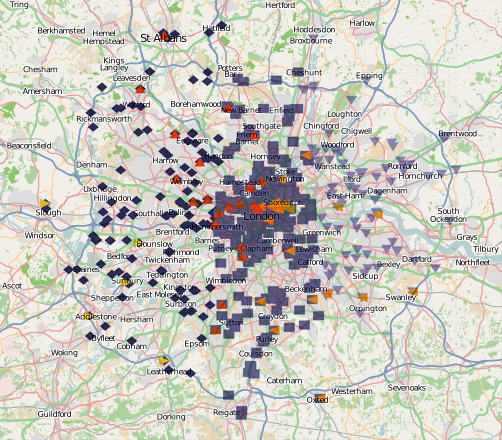
\includegraphics{images/futurework/map_london.jpg}
\caption{Results for clusters at timeslice 9:00 - 10:00am.}
\label{fig:clusters}
\end{figure}

In the above image, we can see a representation of the static clusters and the
timeslice clusters created from tweets. The static clusters were created for
all days for the timeframe of 9:00 - 10:00am, and the slice clusters are
created for the same time at the 29th of February 2012. In the image the three
clusters with tones of blue are the static clusters, and the three clusters
with tones of orange are the timeslice clusters.

The clusters are named from Static 1 to Static 3 and Slice cluster 1 to Slice
cluster 3 from left to right. The K-L divergence gave the following results:

\begin{center}
    \begin{tabular}{| l | l | l | l |}
    \hline
    & Slice cluster 1 & Slice cluster 2 & Slice cluster 3 \\ \hline
    Static 1 & 0.631128807559 & 0.309354831342 & 0.626666260517 \\ \hline
    Static 2 & -0.277093691689 & -0.598627406567 & -0.281078383944 \\ \hline
    Static 3 & -0.0722968487598 & -0.394347406928 & -0.0772419848337 \\ \hline
    \end{tabular}
\end{center}

Given these results we can consider that slice cluster 1 and 3 fall in the
normal behaviour of static cluster 3, but slice cluster 2 seems to suggest a
different behaviour from the static clusters and so could mean a rare event.
If our data were only about traffic could suggest a traffic accident for
example, and this is how it can be used in the future.

\subsection{Gamification}

\subsection{Further enhanced on the classification}
There are multiple ways that can improve the classifier. However, because of the strictly deadline of the project the time wasn�t enough to test all the possible improvements. Therefore the team decided to focus on the other parts of the project. One way to improve classification performance is to combine several classifiers. This can be easily be done by letting the multiple classifiers to use voting, and choose whichever label gets the most votes. For this style of voting, it's best to have an odd number of classifiers so that there are no ties. The individual classifiers should also use different algorithms. For example the Na�ve Bayes, the SVM and another classifier e.g a Decision Tree classifier can vote for a tweet and an algorithm can be used in order to classify the tweet accordingly.  Another way to enhance the classifier is to manually label more data and train the classifier from the beginning. Finally, the inclusion of trigrams collocations could increase the accuracy of the classification.  

\subsection{Analysis of other sources}
As the aim of this project is providing information to the user about traffic disruptions, more sources can 
easily be used for acquiring more information about disruptions in London and other areas. Such examples 
of sources would be news reports published in various websites. These reports could include accidents, general traffic or even 
bad road conditions due to the weather. Moreover, there exist TfL Twitter bots that frequently tweet
about traffic disruptions. Another source that can be used is Facebook. Data regarding traffic can be
extracted from posts, comments or even public groups whose current location is London.

\subsection{Enhanced geocoding}
Various methods exist that can improve the geocoding system implemented in our project. One technique, is extending the geocoding algorithm to recognise tweets written in languages other than English. In addition, advanced regular expressions can be added for extracting street addresses from tweets with a specific or wide range of formats. A more advanced geocoding system could also be implemented using classifiers. These classifiers can be trained with local addresses and be used to resolve locations from complex tweets. More classifiers can be created firstly to detect the language of the tweet and secondly to extract its location context that will be used to retrieve latitude and longitude points.

\pagebreak

\section{Appendix}
	\subsection{Included libraries}
    \subsubsection{Server}

\begin{description}
    \item[Flask] \url{http://flask.pocoo.org/} \hfill \\
        Provides a REST API used for the server.
    \item[pg8000] \url{http://pybrary.net/pg8000/} \hfill \\
        Provides functions used for PostgreSQL.
    \item[NLTK] \emph{Natural Language Toolkit} \url{http://code.google.com/p/nltk/} \hfill \\
        Provides tools used for the classifier.
    \item[python-twitter] \url{http://code.google.com/p/python-twitter/} \hfill \\
        Provides Twitter search functions.
    \item[tldextract] \url{http://pypi.python.org/pypi/tldextract/0.2} \hfill \\
        Finds a domain name from a url.
    \item[googlemaps] \url{http://pypi.python.org/pypi/googlemaps/} \hfill \\
        Provides reverse geocoding from Google Maps.
    \item[OSGB36toWGS84] \url{http://hannahfry.co.uk/2012/02/01/converting-british-national-grid-to-latitude-and-longitude-ii/} \hfill \\
        Module providing conversion between the national British grid coordinates and longitude, latitude coordinates.
\end{description}

\subsubsection{Client}

\begin{description}
    \item[JTwitter] \emph{LGPL} \url{http://www.winterwell.com/software/jtwitter.php} \hfill \\
        Provides Twitter interface.
    \item[oauth-signpost] \emph{Apache Licence 2.0} \url{http://code.google.com/p/oauth-signpost/} \hfill \\
        Provides Oauth authentication for connecting Twitter acounts.
\end{description}


\subsection{Client user interface}
    \begin{figure}
\centering

\mbox{\subfigure{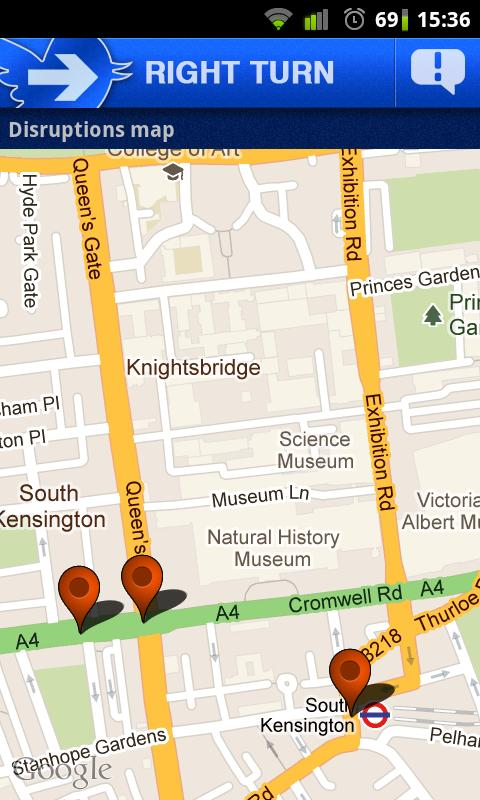
\includegraphics[width=0.4\textwidth]{images/appendix/user_interface/map_view.jpg}
\quad
\subfigure{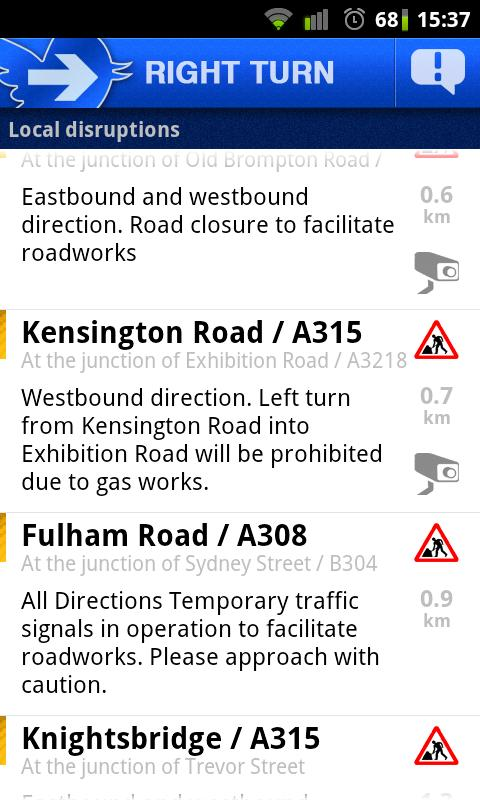
\includegraphics[width=0.4\textwidth]{images/appendix/user_interface/list_view.jpg} }}}


\mbox{\subfigure{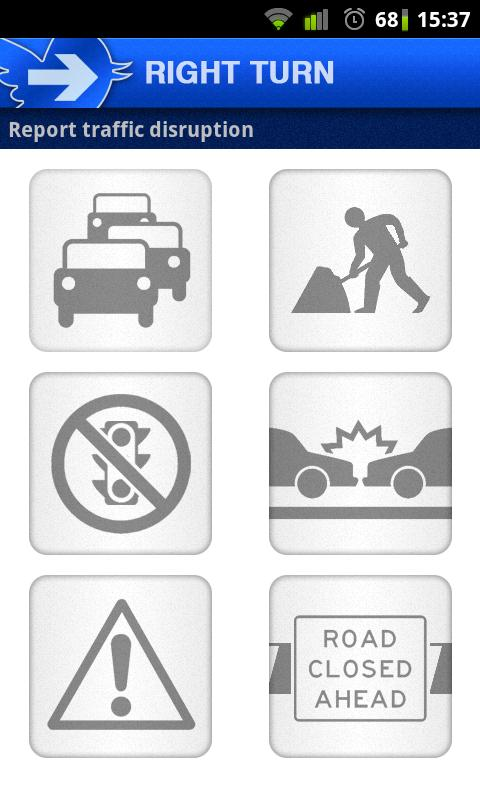
\includegraphics[width=0.4\textwidth]{images/appendix/user_interface/report_view.jpg}
\quad
\subfigure{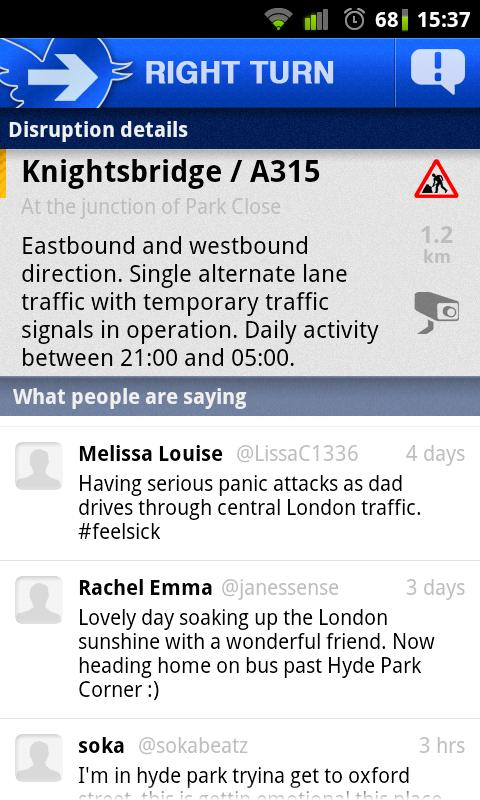
\includegraphics[width=0.4\textwidth]{images/appendix/user_interface/details_view.jpg} }}}

\caption{Examples of the implemented user interface}
\label{fig:user_interface}
\end{figure}

\begin{figure}
\centering
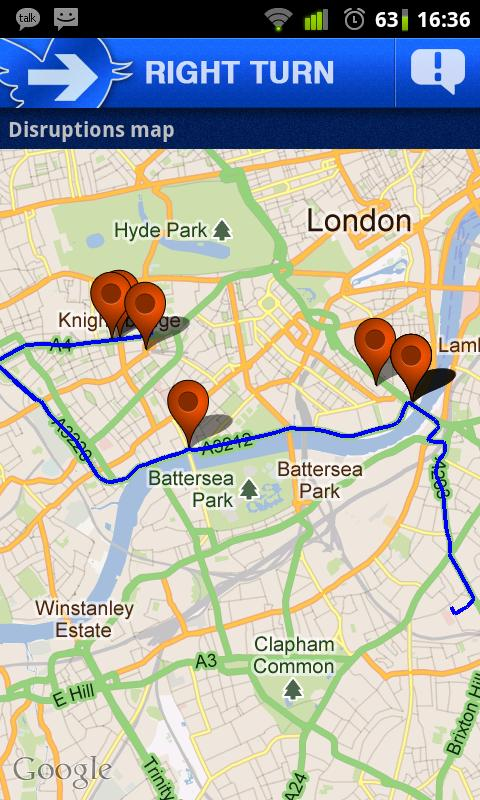
\includegraphics[width=0.45\textwidth]{images/appendix/user_interface/home_route.jpg}
\caption{Example of home route functionality}
\label{fig:home_route}
\end{figure}


\subsection{Online resources}
    \begin{description}
    \item[Github] \url{https://github.com/johnflan/Twitter-4-Traffic/} \hfill \\
        Revision control system.
    \item[Video Demonstration] \url{http://www.youtube.com/watch?v=LmWDxq2jhNI/} \hfill \\
        Video demonstration of the final product.
\end{description}


\pagebreak	
\section{References}
	\vspace{-20pt}
	\def\refname{}
	\bibliography{references}
	\bibliographystyle{plain}

\end{document}
